This chapter outlines our efforts to establish a direction in the domain of technologically mediated personal financial management in the home. The interviews and workshop presented in this chapter constitute the empirical foundation for our understanding of the domain. The interviews seek to create initial insights into how the users handle financial management with a focus on behaviors in the home. The workshop focuses on how the users handle their finances in the home but additionally provides insights into how the attendants would like future banking experiences to feel like and be integrated in the home.

\section{Preliminary Interviews}
This section presents three preliminary interviews that were conducted in the early stage of this project. Each interview aimed to obtain some general knowledge about (our target group’s) financial habits, behaviour and value-set. We conducted an interview with a financial adviser, a woman living with her husband and two kids, and a young couple living together. All interviewees are anonymized in order to maintain integrity and the main findings from these interviews are presented in separate sections. The interview with the financial adviser was held in person and documented using voice recording and notes, while the interviews with our target group members were conducted via Skype using screen recording and phone using voice recording, both complemented with notes. The interview guides used for the interviews can be found in appendix~\ref{app:interview-guide-financial-adviser,app:interview-guide-families}.

\subsection{Financial Adviser}
Prior to the interviews with our target group we conducted an unstructured interview \cite[chapter~7]{sharp2007interaction} with Michael; a 34-year-old senior adviser from Danske Bank with more than ten years of experience within financial counselling. The primary goal of the interview was to gain an overall understanding of how people manage their finances on a daily basis, and how the relationship between a financial adviser and an ordinary customer is currently functioning. The interview lasted around 40 minutes.\\

After the introduction and the warm-up questions our main session started, and after some time it became relatively clear that many of the answers to our questions resided in the advancement of technology. Before his job at Danske Bank, Michael worked at a smaller bank and he described how he, on a daily basis, had more personal contact with the customers. He mainly ascribed this difference to the amount of financial services offered to customers of Danske Bank, as they now have the opportunity to handle simple financial tasks on their own. Even though it might seem a bit contradictory at first the wide range of services available to bank customers has resulted in a higher focus on customer care as the financial advisors no longer have to perform the same amount of trivial tasks. As Michael describes it: \emph{“a lot of our things [daily tasks] have changed because of IT solutions, I mean, the customers can actually do a lot [economic related tasks] at home”}.
During our interview we also asked what he saw as the main reason for unfortunate economic situations and how this could lead to an unhealthy economy. In his perspective undesirable economic situations were often caused by a lack of framing (no budget), and the fact that future projections are difficult to make. Another, yet very important, aspect is how new (young) customers decide on which bank they want to take care of their money. Michael told us about how some people have chosen Danske Bank due to its financial services: \emph{“many customers have opted for Danske Bank because of it [technological services], as others [banks] do not offer as advanced solutions”.} Seeing how banks keep pushing new features to their digital platforms and how customers embrace these features by fast adoption, lead us to believe that self-service and customer empowerment are two key factor in future banking.

\subsection{Family Mother}
We conducted a semi-structured phone interview \cite[chapter~7]{sharp2007interaction} with Charlotte, a 28-year-old woman living in Western Jutland, Denmark, with her husband and two children. Charlotte works a part time job as a nurse and her husband works full time as a mason. The phone interview was performed on a Thursday morning and took approximately 45 minutes.

When asked to describe her economy, Charlotte quickly focused on the changes that had happened economically between her life as a student and a nurse. She used to plan for grocery shopping and make detailed budgets but has become unstructured in this regard as her priorities have changed: \emph{“back then when we had no money we were really good at prioritising. I used to look in offer catalogs, do meal planning and all those things but it all just went out the window”}. She now values vacations with her family highly and describes how they will even take unpaid leave to go on long trips. Her economic values and behavior have changed dramatically with the change in her life situation -- that is having kids and a reliable source of income.
Charlotte values everyday financial insights because it makes her feel in control. She logs into her online bank daily to check up on transactions and make sure that everything is going according to the plan. She confirms that the correct amounts are withdrawn from her account for the purchases she makes and that her salary is deposited to her account. \emph{“For example just an hour ago, I ordered some new clothes for the kids online and then I go to see how it is going [on the netbank] quite instinctively. I do this because i like to be in control of the situation”}. Although Charlotte checks her transactions daily she does not calculate her weekly or monthly expenses in order to adjust her spending behavior but rather makes the adjustment based on intuition after glancing through her transactions. This habit of adapting her spending behavior reactively based on intuition is a way for her to stay in control after she stopped making budgets and knowing exactly how their money was spent.
Charlotte always uses her smartphone or iPad when interacting with her netbank. She leads a busy life so she goes online in quick sessions in between household tasks and as such fits her banking activities into the flow of her everyday life: \emph{“I often log on at the kitchen table. I would say that i am almost never sitting in the couch. We lead busy lives, when the kids are put to bed I have to do the laundry for example and then I will often sit at the kitchen table for five minutes [on the netbank]”}.

\subsection{Young Couple}
Our last interview was a semi-structured with Hanna, a 25-year-old woman working as a physiotherapist, and her boyfriend, Christian, who used to work as a physiotherapist but now pursues a career as a pre- and middle school teacher. They live together in Aalborg which is located in Northern Jutland in Denmark. The interview was conducted via Skype with screen and audio recording and lasted approximately 50 minutes.\\

When asked to characterize their financial situation Hanna and Christian described it as shaky as they currently found themselves in a transitional phase in life with a fluctuating number of work hours and career change, yet they felt comfortable and in control. In contrast to Charlotte (from the previous interview), Hanna and Christian do not have a shared economy. They, however, have a number of shared expenses such housing costs and groceries, therefore they have set up an account for this purpose; they deposit a fixed amount of money every month and the shared expenses get withdrawn from there. Hanna hinted that this kind of solution kept them from arguing about financial matters: \emph{“We deposit money each month for the shared expenses, so we don’t have to discuss how much we [individually] have to pay”}. Later on in the interview, when asked how much time they spent on financial doings, Hanna underpinned this statement by saying that the subject of economy was perhaps not the most pleasant thing to talk about. Approximately once a week they go online to check up on their finances and they usually do this from an iPad or laptop. They make a quick glance at the transactions and from there go to e-Boks (an online mailbox used by the Danish government and some public/private companies) to cross reference with received bills and paychecks. By the end of the month the amount of financial checkups increases in order to make sure they stay within their spending limits. Christian told us he uses a Visa Debit card (a non-credit card) and when asked if it was a way to avoid overspending he responded \emph{“Yes exactly -- I am more comfortable with that.”}. Because of their varying income they sometimes have to borrow money from one another and to keep track of their financial outlays they use a whiteboard located in the living room. They also use a big calendar and notes to keep track of their finances. They use these low-level tools to remind themselves of economy related deadlines and to keep each other informed at all times.

\section{Workshop}
This section presents the exploratory workshop that we conducted to gather further information about people’s financial habits and value-sets related to a domestic context and more importantly to obtain insights into how people would imagine future banking experiences to unfold; both in terms of functionality and interplay between the context and technology. The workshop was carried out in two parts. The first being a series of warm-up exercises and the second work with a self-developed kit, that we call Exploration Kit, which was designed to help participants explore and express their ideas.

The first half of the workshop was spent doing four exercises related to interactions with and feelings about economy. The point of these exercises was twofold; firstly it made the participants reflect upon their own economy in order to create a basis for ideation with the Exploration Kit and secondly it acted as a way to gain knowledge about the participants’ attitude towards economy and usage of current banking tools. The second half of the workshop was assigned to work with the Exploration Kit. The purpose of the kit was to enable the participants to come up with ideas for banking experiences in the home. Importantly the kit forced the participants to not only think of an abstract concept but also how it could be physically manifested in the home context.

The workshop was conducted in the evening and had a duration of approximately 2 hours. Ten people participated in the workshop, seven of which were male and three female. The ages ranged from 22 to 27 and the majority (seven out of ten) had a cohabitant or lived together with one or more people. All of the participants except one were university students and a little more than half of the students had a technical background whereas the other half was less tech-savvy.

\subsection{Warm-Up Exercises}
In order to establish an inspirational atmosphere and spark creativity we conducted a series of introductory exercises. These exercises aimed to capture some general knowledge about the participants’ background, technology usage and financial attitude. Many of the exercises were designed in the spirit of Gaver et. al’s Cultural Probes \cite{gaver1999design} as they strived to capture data in a more inspirational and imaginative manner.

\begin{figure}[!h]
	\centering
	\includegraphics[width=\textwidth]{warm-up-exercises}
	\caption{\textbf{Top left:} Some of the pictures created during the \textit{Draw your economy} exercise. \textbf{Top right:} Floor plans created in the \textit{Floor plan} exercise. \textbf{Bottom left:} Sequence of emoticons used to describe the emotional relationship with money in the \textit{Emoticonometer} exercise. \textbf{Bottom right:} Ballot papers from the \textit{Voting} exercise.}
	\label{fig:warm-up-exercises}
\end{figure}

\subsubsection*{“Draw Your Economy”}
We initiated the workshop with the task to “draw your economy”. This exercise was very much inspired by Kaye et al. \cite[p.~522]{kaye2014money} and was intentionally very open as the participants were told they could draw whatever came into their minds. The goal of the exercise was to make the participants reflect upon their own economic situation in order for them to use this as a foundation for the later ideation with the Exploration Kit. Furthermore, it gave us insights into the participants’ mindsets towards economy.

The drawings can generally be divided into two categories. The first category contains abstract drawings that try to convey the feeling the person is experiencing in relation to their economy, e.g. a man standing on top of the world or a man struggling to find water in the desert (see figure~\ref{fig:warm-up-exercises} top left picture). The second category contains more concrete and diagrammatic drawings related to spending or the money flow, e.g diagrams showing the spendings account balance over time or diagrams showing how the monthly income is spent in relation to different categories such as housing costs, leisure and groceries. Some participants combined the two categories to convey their general feelings or mindset about economy while also hinting at how they spend their money. One participant, who combined the categories, drew a person floating down a river (a stream of money) surrounded by food, gifts, clothes and so on.

The ways the participants think about economy and spend money are numerous. However, there is a tendency towards an either very positive or negative attitude regarding economy. Some participants portray their economy as struggling or unstable while others display joy and satisfaction. One participant drew himself on top of the world and explained that he was a big consumer and very deliberately purchased items related to his hobby which would result in positive emotional responses such as excitement or happiness. It was a common theme for people who had a positive attitude to focus on the possibilities and explicitly what made them happy. One participant valued holidays highly, another clothes and a third computer games and equipment. A participant with a negative attitude drew the Leaning Tower of Pisa and explained that he thought his economy was off balance because he did not care much about it and at times completely neglected it. Common for the ones with a negative attitude was the general dislike of economy as a subject and frequently neglecting it.

\subsubsection*{Floor plan}
In order to get a better understanding of how people organize and interact with their economy in the context we asked them to draw a floor plan of their residence and place different markers, representing various technologies or mediums, on this floor plan.
As financial information is accessible from many different platforms, it comes as no surprise that information is not strictly bound to specific artifacts or locations. The artifacts used ranged from simple paper and Excel spreadsheets to the more multipurpose smartphone. Looking at the floor plans created during the workshop it becomes evident that the increased portability in digital devices has altered the way we connect with our economy and shows that – even though we are not completely aware of it – financial interactions are more omnipresent than ever before. Most of the participants used laptops, tablets and smartphones as a way to stay in touch with their economy, and no place in the home seemed to be “sacred”. The living room, kitchen and the bed seem to be most popular places to interact with economy, however only very few restricted their interaction with money to very specific places or rooms.

\subsubsection*{Emoticonometer}
In one of the exercises we asked the participants to express how they felt about their financial situation. Inspired by the Smileyometer \cite{read2006using}, we provided the participants with a set of emoticons and asked them to answer three questions, e.g. “how is your relationship with the bank”, using these emoticons. We decided to use emoticons instead of hand drawn smileys as we feel the average user, having varying drawing skills, will be able to express their emotional state towards economy more precisely. Also, since the emoticons embody a wider and more diverse range of emotions it can no longer be characterized as a traditional Likert scale. With this exercise we hoped to gain a better understanding of how people are emotionally engaged in different aspects of their economy and where there might be an opportunity for improvement. Based on the output from the workshop we see that people have mixed feelings about their economy (see figure~\ref{fig:warm-up-exercises} bottom left picture). The participants used very different emoticons for the same questions, however most of the participants used a somewhat positive emoticon to express their personal economy, whereas the topic of talking economy with others and the relationship with the bank were more diverse. This is very much in line with the first exercise where people drew their financial situation.

\subsubsection*{Voting}
In the last exercise we asked the participants to fill out a ballot paper (see figure~\ref{fig:warm-up-exercises} bottom right picture) where they indicated any technology they had used to manage their personal finances on that particular day. This resulted in the following distribution:

\vspace{12pt}
\begin{itemize}
	\item E-bank: 1
	\item Mobile e-bank: 3
	\item MobilePay: 5
	\item Creditcard: 8
	\item Cash: 1
	\item WeShare: 1
\end{itemize}
\vspace{12pt}

A clear pattern emerges showing that the old “technology” in the form of cash is on the retreat while the well established credit card technology is still the most prevalent. However, we see a rise in the adoption of new solutions namely MobilePay and mobile e-banking, which resonates well with the current trends of digitization. In this regard it is important to take the participants under study into account particularly their relatively young age. While young people are known to adopt new technologies faster, we believe that it is also part of a general tendency towards more rapid technology adoption.

\subsection{Exploration Kit}
In the second part of the workshop we introduced our Exploration Kit (see figure ~\ref{fig:exploration-kit}) which has been inspired by Rodden et al.s ‘physical jigsaw editor’ prototype \cite{rodden2004between}, where jigsaw pieces are used to build sequences as a way to compose various technology arrangements in the home. Our kit contains four main categories of pieces in different colors that are combined in a sequence and is meant to make the participants reflect upon various aspects of a new banking experience in a specific order. The categories are designed to help the participants to consider one part of the concept at a time instead of all at once, aiding them in the difficult process of coming up with new ideas and avoiding frustration or confusion. The first category \emph{data type} is concerned with the kind of financial information or action that is desired e.g. transactions or savings. The second category \emph{resolution} is regarding the resolution (level of detail) of the information that is manipulated; low resolution being simple information that is quickly understood but has limited information capacity and high resolution being complex information with unambiguous and detailed information. The third and fourth category is \emph{input} and \emph{output} respectively which deals with the modalities of the interaction and are intended to make the participants consider the physical manifestation and functionality of the concept by asking themselves questions such as \emph{how do you interact with it and what is the outcome?} and \emph{what should it look like and where would I like it in my home?}. Finally, the Exploration Kit contained two optional categories concerned with filtering and triggering of information; filtering being sorting data or selecting specific information to be inspected in more detail and triggering as in deciding when and how information becomes visible. These optional categories were designed to be additional considerations that could be performed after the main sequence was built and the outline of a new banking experience made.

\begin{figure}[!h]
	\centering
	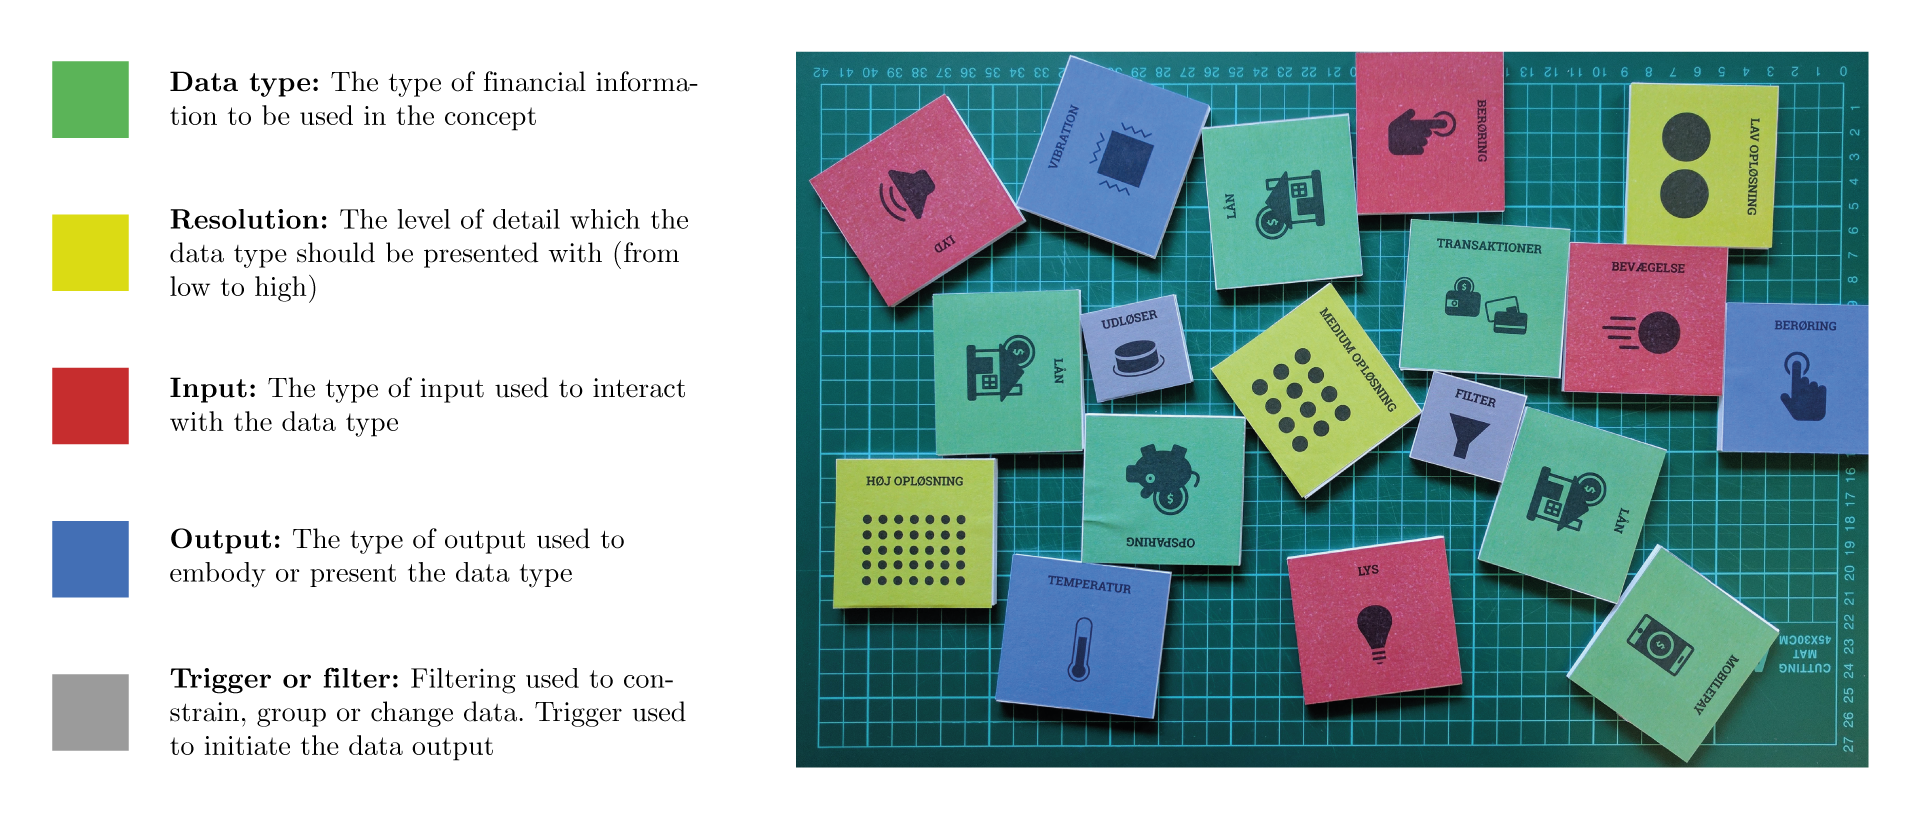
\includegraphics[width=\textwidth]{exploration-kit}
	\caption{Overview of the exploration kit}
	\label{fig:exploration-kit}
\end{figure}
\subsubsection*{Provotypes}
The Exploration Kit was introduced to the participants along with two “provotypes” \cite{boer2012provotypes} that we created using the kit ourselves. These provotypes acted as an introduction to how the Exploration Kit should be used while also creating provoking thoughts on how financial technology in the home could look like. It was crucial for us that the provotypes were perceived as slightly odd or unconventional in order to instill a sense of creative freedom in the participants -- it was perfectly acceptable and desired to come up with silly ideas. One of the provotypes we presented was a scale (see figure ~\ref{fig:provotype}) to “weigh” financial transactions and get information on spendings in different categories. A cube with category-labels such as \emph{clothes} and \emph{transport} on the sides is placed on the scale to weigh the spendings in the category facing upwards. A bar on the scale indicates how much of the monthly budget that has been spent in the selected category, i.e. if the bar is 25 percent full it means 25 percent of the total monthly budget has been spent in that category. As stated we used the Exploration Kit in the creation of the provotype; the point of departure was the selection of transactions as the data type and a medium data resolution as we wanted the possibility to manipulate and explore the information to some extent. Thinking of the input category and consequently the interaction, we decided that touch or pressure would make for an interesting and alternative experience. Based on these constraints we started brainstorming on touch sensitive objects and interactive pressured based surfaces ultimately leading to the idea of a kitchen scale and the concept of weighing your economical transactions. Finally, we decided on light as an output in the form of a LED display that shows the relative spending in a given category.

\begin{figure}[!h]
	\centering
	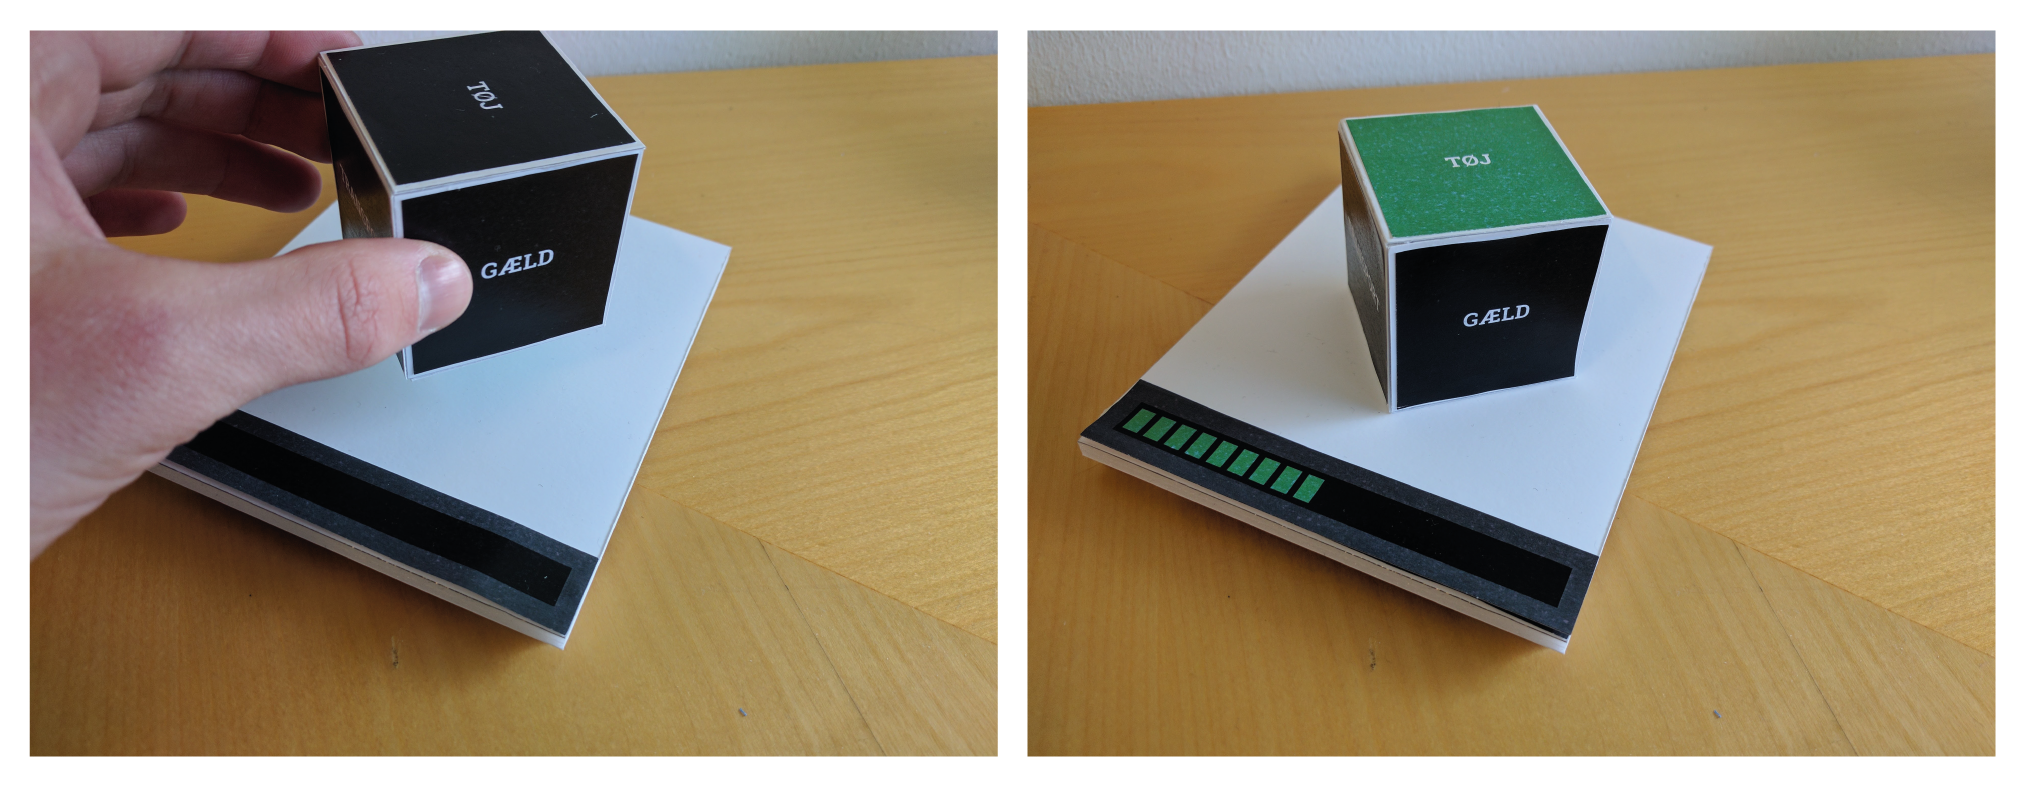
\includegraphics[width=\textwidth]{provotype}
	\caption{Kitchen scale provotype used to provoke and inspire the workshop participants}
	\label{fig:provotype}
\end{figure}

\subsubsection*{Working with the Exploration Kit}
In order for the participants to be more expressive we provided them with an assortment of materials (pen, paper, balloons, play dough, etc.) which they could use to externalize their ideas. In average each participant created two ideas using the kit of which many reflected some kind of personal experience with economy.

\begin{figure}[!h]
	\centering
	\includegraphics[width=\textwidth]{working-with-exploration-kit}
	\caption{\textbf{Top left and right:} Participants working with the exploration kit. \textbf{Bottom left:} AI robot created by one of the workshop participants. \textbf{Bottom right:} Talking one-dollar bill concept created by one of the workshop participants.}
	\label{fig:working-with-exploration-kit}
\end{figure}

One of the participants told us that he would often forget to read messages from the bank, therefore he envisioned a refrigerator magnet shaped like a one-dollar bill where a talking George Washington would read messages from the bank aloud (see figure~\ref{fig:working-with-exploration-kit} bottom right picture). Another participant also used an avatar-like data representation, however in a much more indirect and subtle manner. He imagined his finances represented as a fish in an aquarium and depending on the color and the behaviour of the fish as well as temperature and flow of the water would be able to infer the state of his finances. This idea stemmed from the fact that he spends many hours at a desk, therefore he pictured this kind of representation to be suitable and playful. Even though this kind of solution is simply an alternative representation of financial data, it will most likely induce a more reflective practice in relation to spending habits. One of the participants knew he would often spend money on what he called “stupid things” and therefore he designed a wallet with a built-in screen that would prompt him every time he bought something above a certain price tag. This type of enforced evaluation was not found among the other participants’ designs, yet some degree of quality assessment could be seen, e.g. represent financial status through colored light. A more radical design was an AI (artificial intelligence) robot with a multitude of functionality (see figure~\ref{fig:working-with-exploration-kit} bottom left picture) that was designed to replace the current financial advisers. The participant felt this kind of solution was needed as she had no trust in banks or advisers, and believed that an impartial robot would give her the best financial advices. A different participant developed a concept that did not involve a physical artifact. He envisioned a solution where financial data could be linked to the lighting system of the house (e.g. Philips Hue). Triggered by bodily movement the system would then be able to convey financial information through color and light intensity. Another concept that ended up being a big inspiration for our exploration process was the idea of turning information on and off. The person behind this idea described how financial information would appear/disappear on her wall based on eye tracking. For her, economy is an extremely sensitive matter and therefore she wanted to be in complete control over the visibility of information being conveyed. A recurring theme for many of the ideas was simple data representations (low resolution). Almost all of the participants used low to medium resolution when describing their idea which indicate that comprehensive data representations are reserved for existing solutions such as netbank or other applications.

\section{Data Analysis and Initial Findings}
\label{sec:data-analysis-and-initial-findings}
This section summarises and combines the findings from the preliminary interviews and the workshop into emerging themes that are of particular interest in the domain of financial management technology for the home. We discovered the emerging themes by looking for general tendencies in the data which was achieved through affinity diagramming. Affinity diagramming is a technique where large amounts of data is grouped based on natural relationships and is often used in contextual inquiry as a way to organize insights from field studies \cite{beyer2010user}. The affinity diagram is built bottom up by grouping similar findings and then labeling them, resulting in a structure that reflects the weight of the data rather than our own preconceived thoughts and ideas. We created an affinity diagram for the workshop and one for each interview after which we combined them into one coherent diagram by connecting different data clusters using strings (see figure~\ref{fig:affinity-diagram}). From the accumulated affinity diagram we derived some general themes that will be described in the following sections. Some of the emergent themes are equatable or related to the research areas presented in chapter~\ref{ch:framing-the-domain} and therefore serve as a validation of the relevance in our domain.

\begin{figure}[!h]
	\centering
	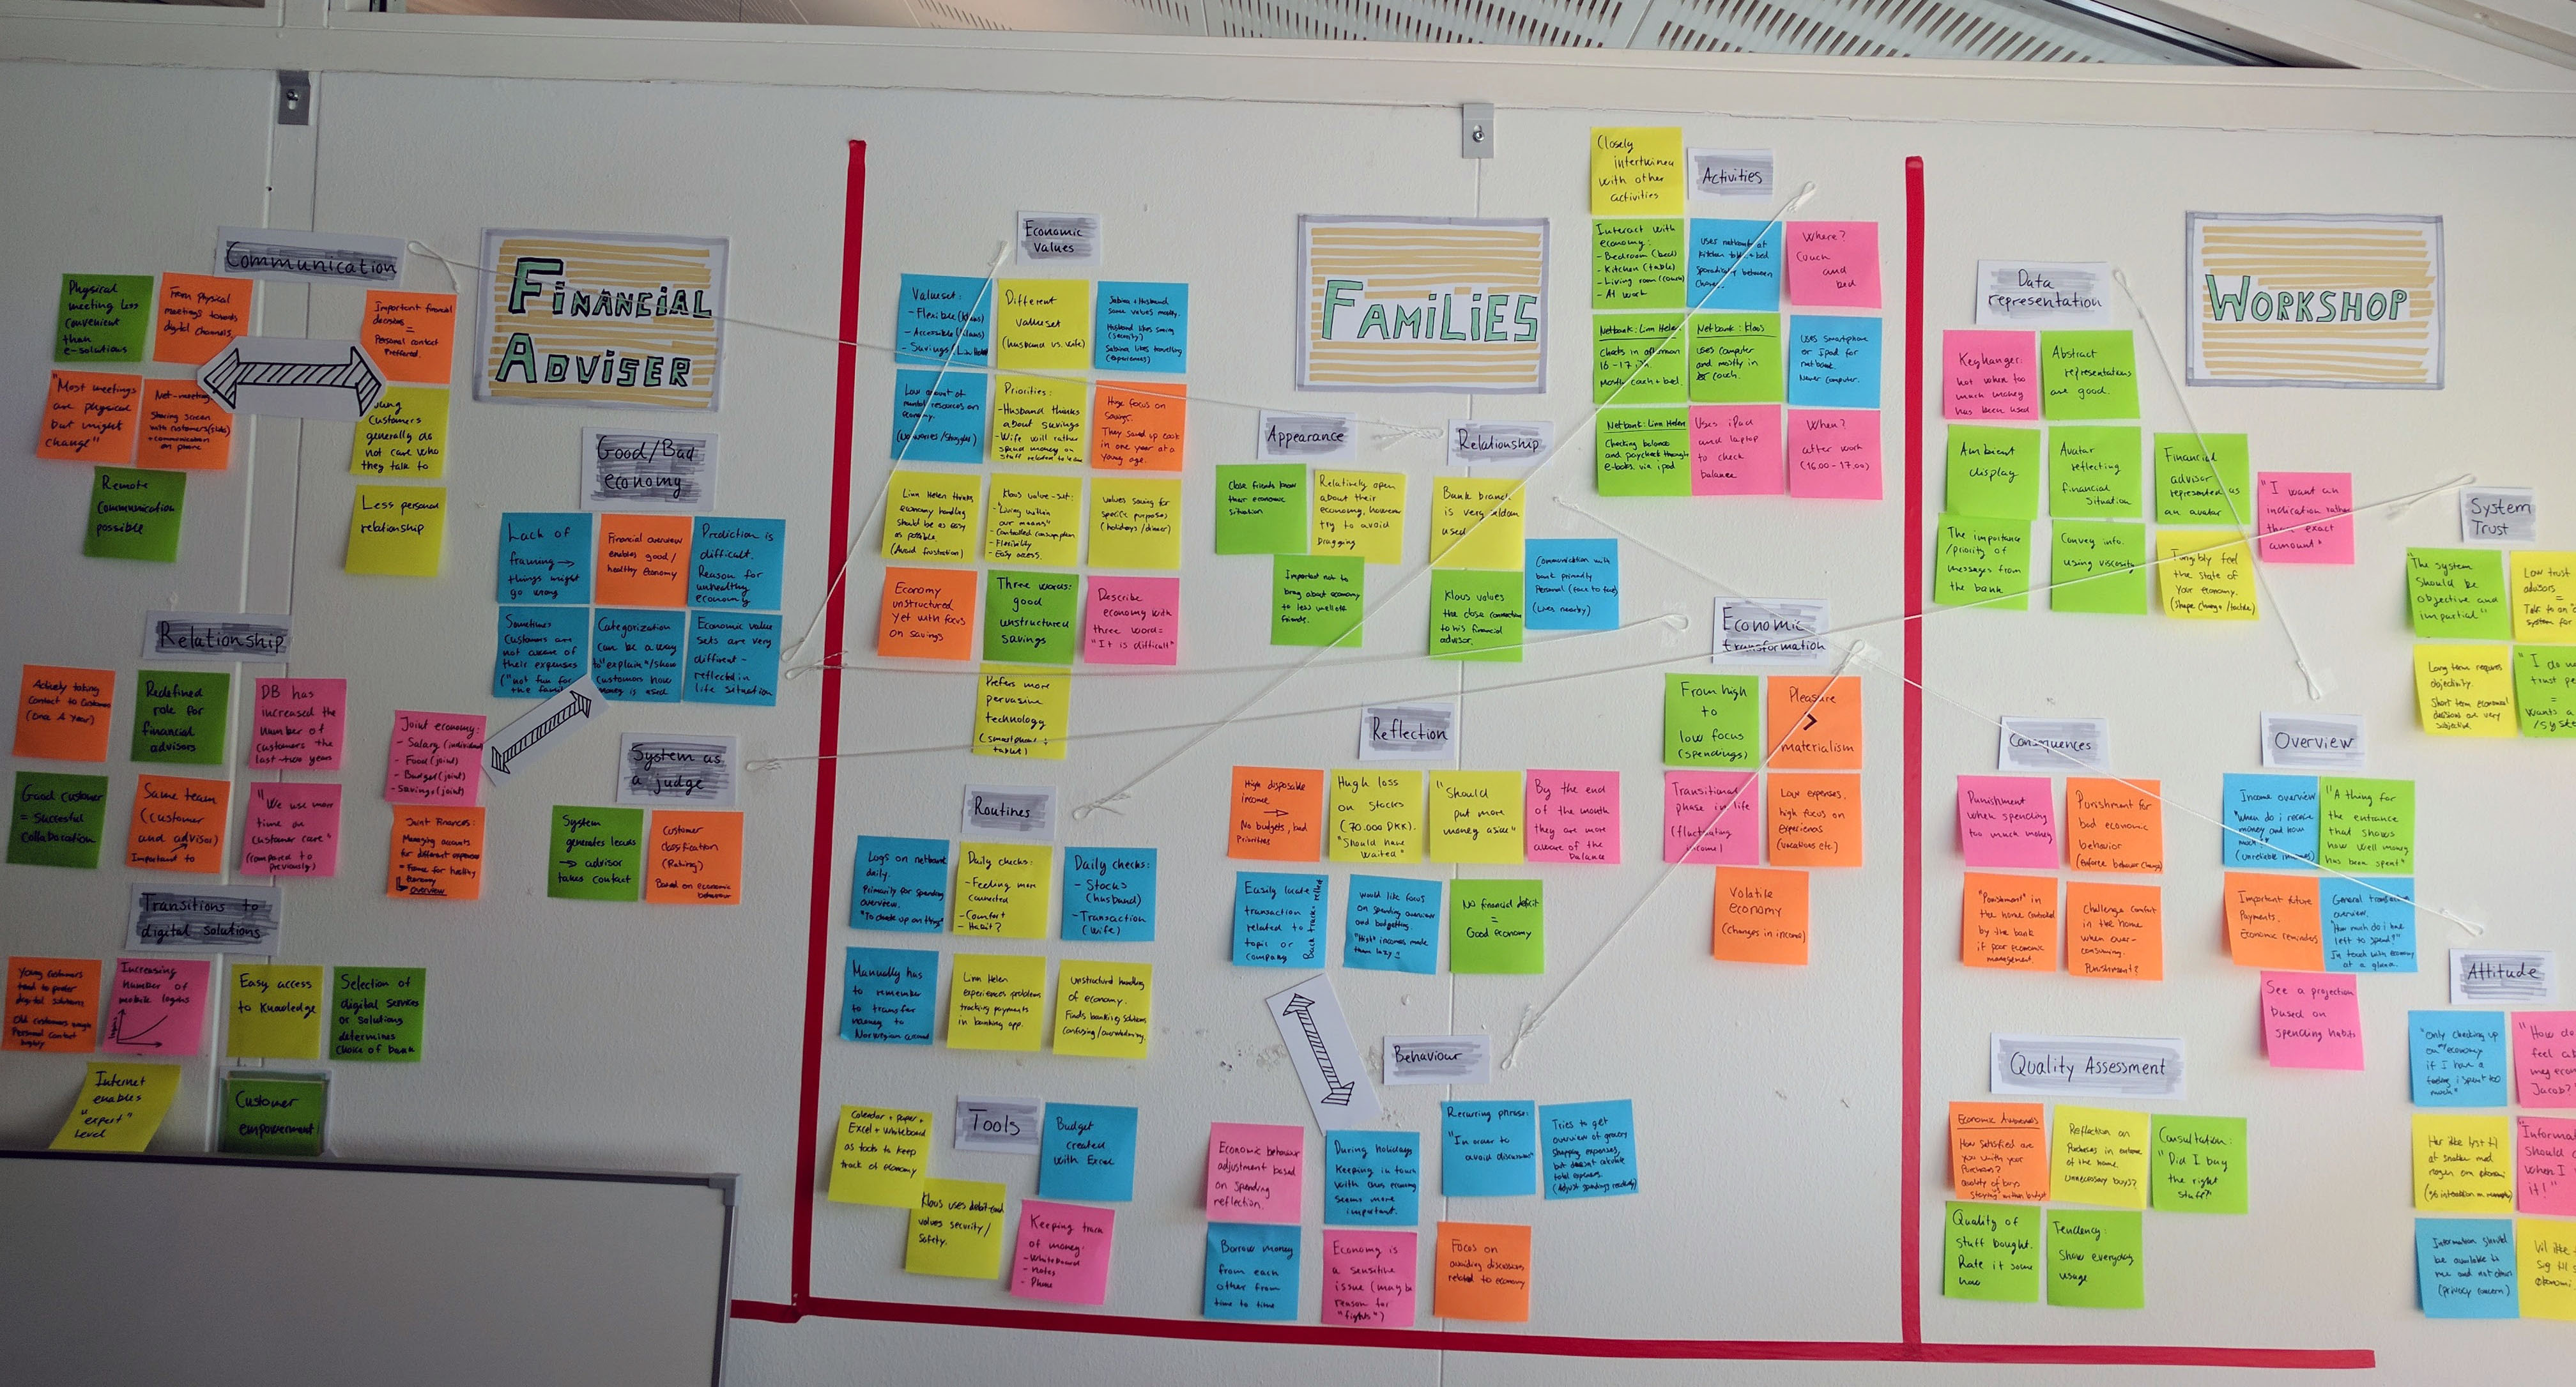
\includegraphics[width=\textwidth]{affinity-diagram}
	\caption{Accumulated affinity diagram created based in the preliminary interviews and the workshop}
	\label{fig:affinity-diagram}
\end{figure}

\subsection{Portability}
The first theme is based on the interplay between the existing ecology of technologies and contextual behaviours (i.e. routines). As reported in the floor plan and voting exercises users utilize a wide array of tools when seeking out and managing financial information. Many of these tools (e.g smartphones or tablets) are portable and can be used at different locations in the home (bed, kitchen table, couch, etc.). This exemplifies that spatial freedom, more specifically the ability to undertake tasks anywhere, has become of high value among many users. Due to their portability many of these devices can be integrated into existing routines but can also provide a foundation for new ones. In the interview with Charlotte we found that she had created a routine where she would check up on her finances at the kitchen table in between household activities. The portability of her devices (smartphone and tablet) allowed her to integrate financial activities into her existing routines. The interview with Michael, the financial adviser, revealed that banks are constantly pushing new functionality to their existing applications as customers -- especially young customers -- expect much from the financial services provided by the banks. This shift towards customer empowerment through self-service also led us to believe that providing the users with portable financial technology that can be configured to work with existing domestic technologies and routines serves as a promising direction for further exploration.

\subsection{Seamless Context Integration}
We found the theme of context integration to be recurring in many of the participants’ ideas and concepts in the work with the Exploration Kit. In one of the more radical cases a girl wanted her financial information to be displayed on her wall but only when she glanced at it and was alone in her home. She found economy to be extraordinarily sensitive compared to other personal information and when asked to elaborate on the reasoning behind her idea, she responded: \emph{“I want to make absolutely sure that I’m the only one inspecting my financial information. I think it is very private data that I don’t want to share with anyone”}. Her concept is highly motivated by privacy which explains her wish for the technology to be so integrated in the context that it is able to completely disappear. Other participants valued the aesthetic character greatly, that is, creating a concept that fit stylistically into their homes. Many participants achieved this by making concepts about Interactive Household Objects, i.e. making existing artifacts in their homes “smart”; one participant created a concept with a digitized fish tank where the health of the fish reflected the user’s economic status. Another participant made a concept with a smart key hanger that would brief the user on their economic status as they left the home. These wishes to make the technology at home resonates well with the findings made by Hughes et al. \cite{hughes1998understanding} stating that the aesthetics are important for the technology to be accepted and integrated in the home. We find that designing for a seamless context integration can be a great way to obtain technology adoption and use, especially when designing technology that deals with sensitive data.

\subsection{Daily Routines}
Routines are commonplace in everyday life and they are especially prevalent in the domestic context. As described by Tolmie et al. \cite{tolmie2002unremarkable} in the previous chapter, routines help us get through the repetitive tasks of everyday life by undertaking sequences of practical action without hesitation or mental effort. We see several examples of routinely behavior in both our interviews and the workshop. In the workshop one participant designed a key hanger to get briefed on his economy as he left the house. In this case, picking up the keys at a designated place before leaving the house is clearly part of a routine that is performed to remember certain items. It made sense for him to augment this routine with information about his economic status, as he rarely checked up on his balance. He believed it would help him spend his money more rationally as he would avoid impulsive purchases when his balance was low. In the interview with Charlotte, a family mother, she reported how her banking activities were intertwined with household routines e.g. checking up on transactions in between tucking in the kids and doing the laundry. Christian and Hanna described how they routinely used a whiteboard as a way to coordinate their activities and keep track of their finances. We believe that our findings regarding routinely behavior in the home as well as the literature on designing technology for the home support routines as a theme for further exploration.

\subsection{Data Representation}
In many of the concepts developed during the workshop, simple data representations seemed to be preferred over more complex and detailed ones. A few of the concepts even had a more abstract nature (e.g. showing financial information through a fish and its habitat) which can be viewed as a way to govern sensitive data from the “outside world”. If information is encoded in such a way that the intended receiver -- usually the person owning the data -- is the only one who can make sense of whatever information is visible, then relatively sensitive data can be conveyed without compromising personal privacy. However, this places a higher demand on the receiver as he/she should learn to decode information and do so without too much mental effort. Another important point about the low to medium data representations is that data becomes more perceivable as less information needs to be conveyed. Keeping the information density low decreases the users’ cognitive load and consequently makes information more glanceable. As found in the interviews from the previous sections and the work done by Kaye et al. \cite{kaye2014money}, users tend to engage with finances in very short time periods and when doing so, they make sense of their financial data by looking at transaction patterns and anomalies. Therefore a lot can be gained by working with the data representation in the context of economy.
